\documentclass[a4paper,12pt]{report}
\usepackage[utf8]{inputenc}
\usepackage[francais]{babel}
\usepackage{fancyhdr}
\usepackage{graphicx}
\usepackage{tikz}
\usetikzlibrary{calc}
\usepackage{listings}
\usepackage{xcolor}
\definecolor{grey}{rgb}{0.9,0.9,0.9}
\usepackage{titlesec}
\usepackage{verbatim}
\usepackage{listings}
\usepackage{textcomp}
\usepackage{hyperref}
\usepackage{amssymb}
\usepackage{amsmath}
\usepackage{longtable}
\usepackage{colortbl}
\usepackage{float}
\usepackage{caption}
\usepackage{subfig}
\usepackage{color}


\lstset{ %
  language=R,                     % the language of the code
  basicstyle=\footnotesize,       % the size of the fonts that are used for the code
  numbers=left,                   % where to put the line-numbers
  numberstyle=\tiny\color{gray},  % the style that is used for the line-numbers
  stepnumber=1,                   % the step between two line-numbers. If it's 1, each line
                                  % will be numbered
  numbersep=5pt,                  % how far the line-numbers are from the code
  backgroundcolor=\color{white},  % choose the background color. You must add \usepackage{color}
  showspaces=false,               % show spaces adding particular underscores
  showstringspaces=false,         % underline spaces within strings
  showtabs=false,                 % show tabs within strings adding particular underscores
  frame=single,                   % adds a frame around the code
  rulecolor=\color{black},        % if not set, the frame-color may be changed on line-breaks within not-black text (e.g. commens (green here))
  tabsize=2,                      % sets default tabsize to 2 spaces
  captionpos=b,                   % sets the caption-position to bottom
  breaklines=true,                % sets automatic line breaking
  breakatwhitespace=false,        % sets if automatic breaks should only happen at whitespace
  title=\lstname,                 % show the filename of files included with \lstinputlisting;
                                  % also try caption instead of title
  keywordstyle=\color{blue},      % keyword style
  commentstyle=\color{green},   % comment style
  stringstyle=\color{magenta},      % string literal style
  escapeinside={\%*}{*)},         % if you want to add a comment within your code
  morekeywords={*,...}            % if you want to add more keywords to the set
} 


\frenchbsetup{StandardLists=true}
\newcommand{\marge}{18mm}
\usepackage[left=\marge,right=\marge,top=\marge,bottom=\marge]{geometry}
\pagestyle{fancy}
\setlength{\headheight}{14pt}
\chead{
  \textbf{Binôme :} Douaille Erwan \& François Rémy
  \hspace{2em}
  \textbf{Groupe :} M1 Info RDF}
\renewcommand{\headrulewidth}{1pt}
\linespread{1}
\setlength{\columnseprule}{0.2pt}





\begin{document}


\makeatletter
\begin{titlepage}
\centering
\vspace{-10em}
{\LARGE \textbf{\textsc{Rapport de Projet RVI}}}\\
\vspace{3em}

\includegraphics[scale=0.6]{image/thalassa.png}\\
\vspace{3em}
{\LARGE \textsc{Projet Thalassa: simulation de plongée sous-marine}}\\

\vspace{8em}
Par\\
\vspace{1em}
{\LARGE \@author}\\

\vspace{2em}



\begin{tikzpicture}[remember picture,overlay]

\node [below left,xshift=-1cm, yshift=4cm] at (current page.south east){
\includegraphics[scale=0.6]{image/ustl1.png}};

\end{tikzpicture}
\end{titlepage}
\makeatother

\sloppy

\setcounter{page}{1} 
\newpage

%%%%%%%%%%%%%%%%%%%%%%%%%%%%%%%%%%%% INTRODUCTION
%%%%%%%%%%%%%%%%%%%%%%%%%%%%%%%%%%%%%%%%%%%%%%%%%
%%%%%%%%%%%%%%%%%%%%%%%%%%%%%%%%%%%%%%%%%%%%%%%%%
\section*{Introduction}

Le but de ce TP est de réduire l'espace de représentation en identifiant un axe de projection principal. Entre autre, nous représenterons toutes nos données sur cet axe, ce qui nous permetttra des les différencier. Ici, nous utiliserons l'analyse quadratique linéaire pour classifier les différentes classes.
	
\section*{Question 1}

\begin{lstlisting}
(load(file="x_app.data"))
(load(file="classe_app.data"))
(load(file="classe_test.data"))
(load(file="x_test.data"))

couleur <- rep('red', n_app)
couleur[classe_app==2]='green'
couleur[classe_app==3]='blue'

plot(x_app, col=couleur)
\end{lstlisting}

\begin{figure}[!ht]
	\center
	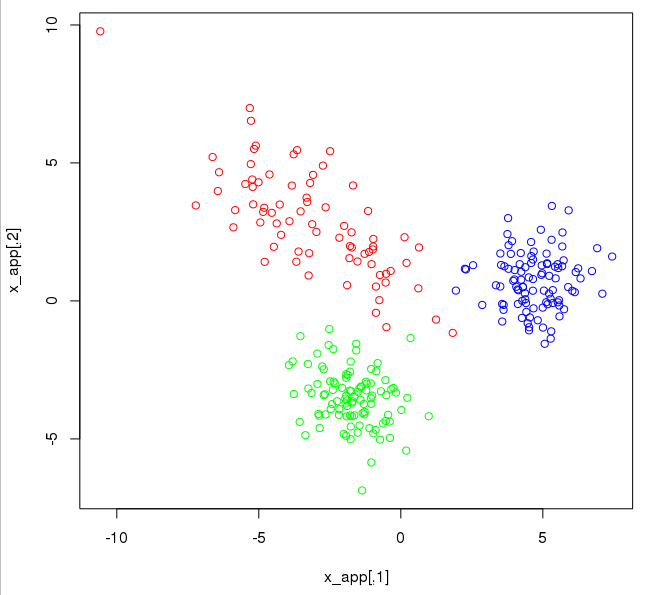
\includegraphics[scale=0.3]{image/q1_1.png}
	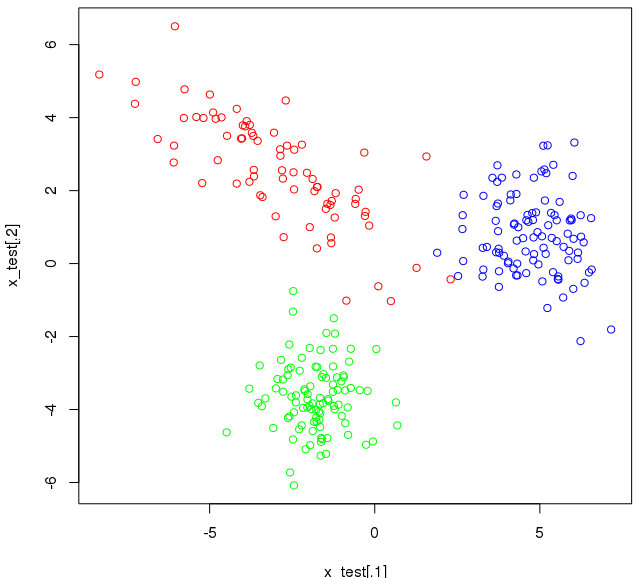
\includegraphics[scale=0.3]{image/q1_2.png}
\end{figure}

À gauche nous avons l'image représentant les données d'apprentissage et à droite les données de test.
On remarque que les données d'apprentissage sont plus centrées pour permettre, surement, d'identifier au mieux les futurs données utilisées. Dans le test on remarque que les données sont proches de celles d'apprentissage et plus éparpillées. 

\newpage

\section*{Question 2}

\begin{lstlisting}

S <- cov(x_test)
Vp <- eigen(S)	

pente <- Vp$vectors[2,1]/Vp$vectors[1,1]
abline(a = 0, b = pente, col = "black")

Scal <- x_app
Scal <- x_app % * % (Vp$vectors[,1]) / sqrt(sum(Vp$vectors[,1]*Vp$vectors[,1]))
XP <- x_app
XP[,1] = Scal * Vp$vectors[1,1]
XP[,2] = Scal * Vp$vectors[2,1]
points(XP[classe_app==1,], col="red")
points(XP[classe_app==2,], col="green")
points(XP[classe_app==3,], col="blue")
\end{lstlisting}

\begin{figure}[!ht]
	\center
	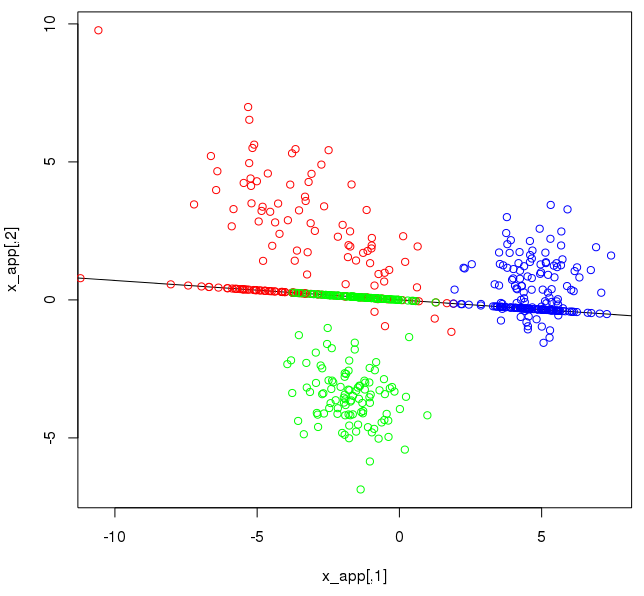
\includegraphics[scale=0.4]{image/q2.png}
\end{figure}

Contrairement aux données de la classe 3 (en bleu), les données des classes 1 et 2, respectivement en rouge et vert, ne peuvent pas être correctement discriminées. On observe que sur la projection les points rouges et verts sont mélangés malgrès que l'on distingue deux zones ayant chacune une couleur dominante. 

\newpage

\section*{Question 3}

\begin{lstlisting}
shape<-rep(1, 301) ;
shape[assigne_app$class==2]=2
shape[assigne_app$class==3]=3
\end{lstlisting}

\begin{figure}[!ht]
	\center
	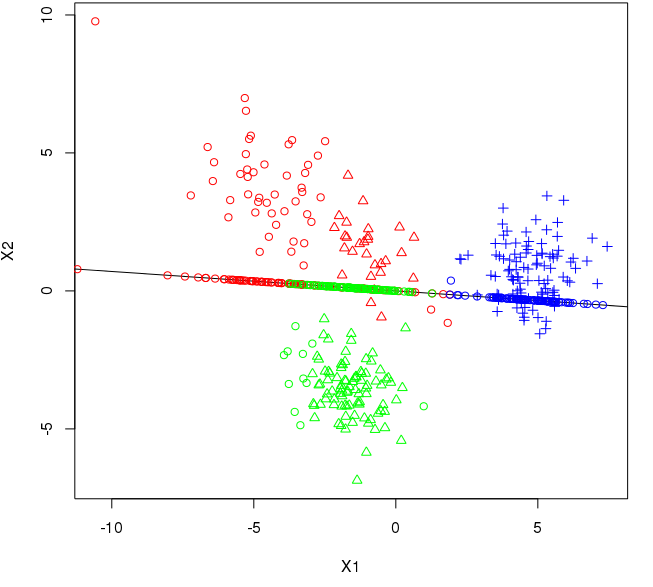
\includegraphics[scale=0.4]{image/q3.png}
\end{figure}

On observe qu'une partie des éléments des classes 1 et 2 (rouge et verte) ont des formes ne correspondant pas à leurs couleurs. Concernant la classe 3, en bleu, le taux de classification est proche de 100$\%$. Cette observation confirme ce que nous avons dit dans la question concernant la distinction possible entre les classes 1 et 2 (rouge et vert).

\begin{lstlisting}
taux_bonne_classif_app <-sum(diag(prop.table(table_classification_app)))
print(taux_bonne_classif_app)
\end{lstlisting}
Le taux de bonne classification des données d’apprentissage projetées sur le 1er axe est de 0.84

\newpage

\section*{Question 4}


\begin{figure}[!ht]
	\center
	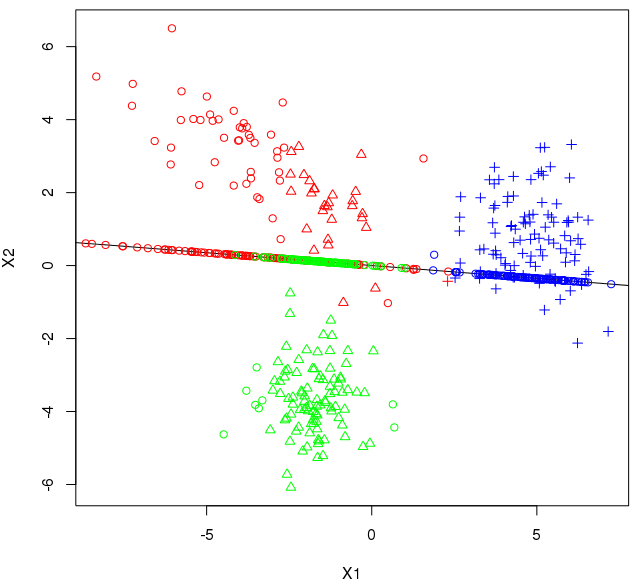
\includegraphics[scale=0.4]{image/q4.png}
\end{figure}

Le taux de bonne classification des données d’apprentissage projetées sur le 1er axe est de 0.85.

La classification n'est pas satisfaisante. On peut constater que certains points appartenant aux classes 1 et 2 sont très dispersés et même mélangés. Le phénomène est visible car des triangles rouges sont mélangés aux cercles rouges. Il en est de même pour la couleur verte.

Avec l'utilisation de ces données on obtient un taux de classification est légèrement supérieur, pourtant les données semble plus dispersées. Il se peut que le fait que les données de classe 1 (rouge) augmente le taux de classification car cette classe est plus éparpillée. 

\newpage

\section*{Question 5}

\begin{lstlisting}
# moyenne classe1
mean1 <- colMeans(x_app[classe_app==1,])
S1 <- cov(x_app[classe_app==1,])
print(S1)
# moyenne classe2
mean2 <- colMeans(x_app[classe_app==2,])
S2 <- cov(x_app[classe_app==2,])
print(S2)
# moyenne classe3
mean3 <- colMeans(x_app[classe_app==3,])
S3 <- cov(x_app[classe_app==3,])
print(S3)

mean <- (mean1 + mean2 + mean3)/3
print("Moyenne")
print(mean)
\end{lstlisting}

La moyenne mean de l’ensemble des données d’apprentissage vaut -0.02314732 et 0.02047070


\begin{lstlisting}
Sw=S1+S2+S3
print("Somme des covariances")
print(Sw)
# covariance inter-classe
Sb=(mean1-mean)*t(mean1-mean)+(mean2-mean)*t(mean2-mean)+(mean3-mean)*t(mean3-mean)
print("Covariance inter classe")
print(Sb)
\end{lstlisting}

Nous obtenons pour la somme des covariances :
\[
   \left (
   \begin{array}{cc}
       7.039024 & -3.480855	\\
      -3.480855 & 5.646092 \\
   \end{array}
   \right )
\]

et pour la covariance inter-classe :
\[
   \left (
   \begin{array}{cc}
       34.7701687 & 0.5952217	\\
      	0.5952217 &  20.9007939\\
   \end{array}
   \right )
\]

\newpage

\section*{Question 6}

\begin{lstlisting}
invSw= solve(Sw)

invSw_by_Sb= invSw * Sb
Vp<- eigen(invSw_by_Sb)

# Affichage de la droite correspondant au vecteur propre
# dont la valeur propre la plus eleve
ScalarProduct <- x_app
ScalarProduct <- x_app  *  (Vp$vectors[,1]) / sqrt(sum(Vp$vectors[,1]*Vp$vectors[,1]))pente <- Vp$vectors[2,1]/Vp$vectors[1,1]
abline(a = 0, b = pente, col = "blue")
XP[,1] = ScalarProduct * Vp$vectors[1,1]
XP[,2] = ScalarProduct * Vp$vectors[2,1]
points(XP[classe_test==1,], col="red")
points(XP[classe_test==2,], col="green")
points(XP[classe_test==3,], col="blue")
\end{lstlisting}

\begin{figure}[!ht]
	\center
	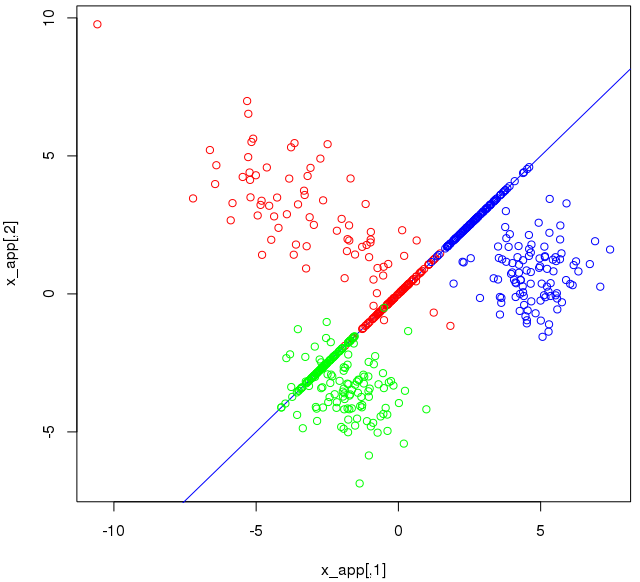
\includegraphics[scale=0.4]{image/q6.png}
\end{figure}

On observe qu'avec cette droite de projection il est plus simple de déterminer les classes. Içi, les classes 1 et 2 (rouge et vert) ne sont plus mélangés et la discrimination peut se faire plus facilement.

\newpage

\section*{Question 7}

\begin{lstlisting}
x_app.lda<-lda(ScalarProduct,classe_app)
assigne_app<-predict(x_app.lda, newdata=ScalarProduct)
# Estimation des taux de bonnes classifications
table_classification_app <-table(classe_app, assigne_app$class)
# table of correct class vs. classification
diag(prop.table(table_classification_app, 1))
# total percent correct
taux_bonne_classif_app <-sum(diag(prop.table(table_classification_app)))
# forme de la classe 1
shape<-rep(1,n_app) ;
shape[assigne_app$class==2]=2
shape[assigne_app$class==3]=3
# Affichage des projections apprentissage classees
plot(x_app,col=couleur,pch=shape,xlab = "X1", ylab = "X2")
abline(a = 0, b = pente, col = "blue")
points(XP[classe_test==1,], col="red")
points(XP[classe_test==2,], col="green")
points(XP[classe_test==3,], col="blue")
\end{lstlisting}

\begin{figure}[!ht]
	\center
	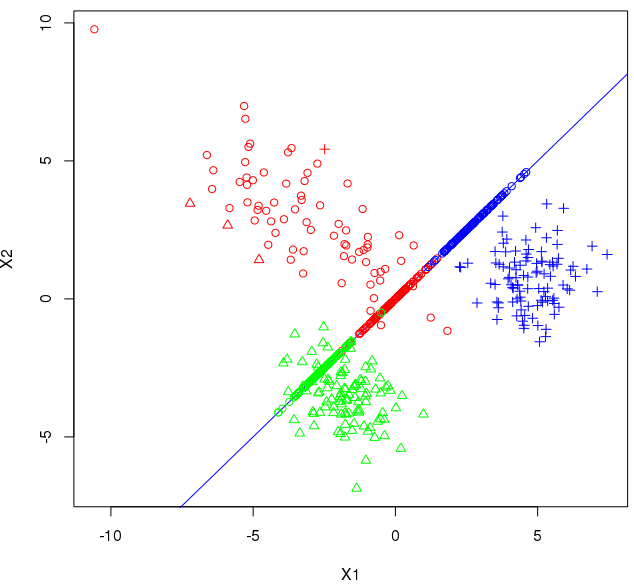
\includegraphics[scale=0.4]{image/q7.png}
\end{figure}

Le taux de bonne classification est de 97.66$\%$. On remarque qu'en effet, certains points sont mal classifiés, mais ceux-ci sont peu nombreux.

\newpage


\section*{Question 8}

\begin{lstlisting}
ScalarProduct2 <- x_test
ScalarProduct2 <- x_test * (Vp$vectors[,1]) / sqrt(sum(Vp$vectors[,1]*Vp$vectors[,1]))

x_app.lda<-lda(ScalarProduct,classe_app)
assigne_app<-predict(x_app.lda, newdata=ScalarProduct2)
# Estimation des taux de bonnes classifications
table_classification_app <-table(classe_app, assigne_app$class)
# table of correct class vs. classification
diag(prop.table(table_classification_app, 1))
# total percent correct
taux_bonne_classif_app <-sum(diag(prop.table(table_classification_app)))
# forme de la classe 1
shape<-rep(1,n_app) ;
shape[assigne_app$class==2]=2
shape[assigne_app$class==3]=3
# Affichage des projections apprentissage classees
plot(x_app,col=couleur,pch=shape,xlab = "X1", ylab = "X2")
abline(a = 0, b = pente, col = "blue")
points(XP[classe_test==1,], col="red")
points(XP[classe_test==2,], col="green")
points(XP[classe_test==3,], col="blue")
\end{lstlisting}

\begin{figure}[!ht]
	\center
	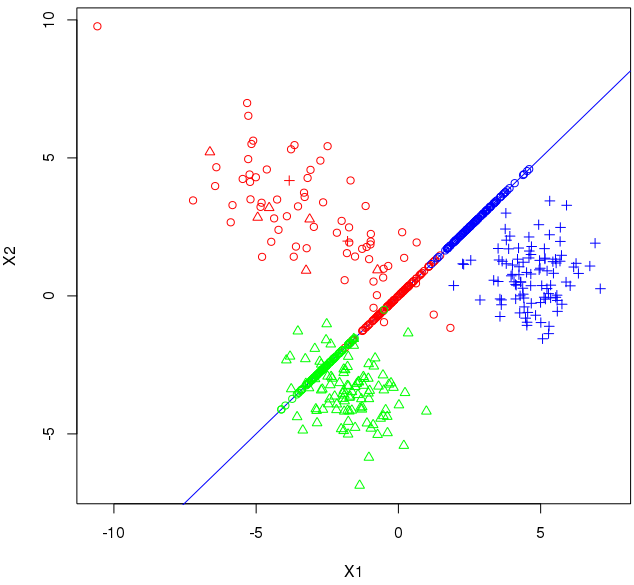
\includegraphics[scale=0.4]{image/q8.png}
\end{figure}

Le taux de bonne classification est de 96$\%$. 

\newpage

\section*{Question 9}
Le taux de bonne classification obtenue par ACP est inférieur que celui obtenu par AFD. Celà s'explique parce que l'axe utilisé en AFD est optimal du fait qu'on indique quelles sont les classes.
Contrairement aux questions de la partie 1 nous avons utilisé l'apprentissage supervisé. L'axe de projection est donc optimal et permet de mieux discriminer, contrairement à notre partie 1 dans laquelle l'axe de projection n'était pas adapté.


\section*{Conclusion}

En conclusion nous avons pu observer différentes méthodes d'analyse, l'analyse par composantes principales et l'analyse factorielle discriminantes. Le mode d'apprentissage de ces méthodes est supervisé, nous avons besoins de données d'apprentissage. L'AFD nous permet de mieux discriminer en mode supervisé que l'ACP. Nous savons donc maintenant que l'apprentissage supervisé est une solution nous permettant de discriminer au mieux les données.


\end{document}
